% Template for Cogsci submission with R Markdown

% Stuff changed from original Markdown PLOS Template
\documentclass[10pt, letterpaper]{article}

\usepackage{cogsci}
\usepackage{pslatex}
\usepackage{float}
\usepackage{caption}

% amsmath package, useful for mathematical formulas
\usepackage{amsmath}

% amssymb package, useful for mathematical symbols
\usepackage{amssymb}

% hyperref package, useful for hyperlinks
\usepackage{hyperref}

% graphicx package, useful for including eps and pdf graphics
% include graphics with the command \includegraphics
\usepackage{graphicx}

% Sweave(-like)
\usepackage{fancyvrb}
\DefineVerbatimEnvironment{Sinput}{Verbatim}{fontshape=sl}
\DefineVerbatimEnvironment{Soutput}{Verbatim}{}
\DefineVerbatimEnvironment{Scode}{Verbatim}{fontshape=sl}
\newenvironment{Schunk}{}{}
\DefineVerbatimEnvironment{Code}{Verbatim}{}
\DefineVerbatimEnvironment{CodeInput}{Verbatim}{fontshape=sl}
\DefineVerbatimEnvironment{CodeOutput}{Verbatim}{}
\newenvironment{CodeChunk}{}{}

% cite package, to clean up citations in the main text. Do not remove.
\usepackage{apacite}

% KM added 1/4/18 to allow control of blind submission


\usepackage{color}

% Use doublespacing - comment out for single spacing
%\usepackage{setspace}
%\doublespacing


% % Text layout
% \topmargin 0.0cm
% \oddsidemargin 0.5cm
% \evensidemargin 0.5cm
% \textwidth 16cm
% \textheight 21cm

\title{Estimating demographic bias on tests of children's early vocabulary}


\author{{\large \bf George Kachergis (kachergis@stanford.edu)} \AND {\large \bf Nathan Francis (nathan99@stanford.edu)} \AND {\large \bf Michael C. Frank (mcfrank@stanford.edu)} \\ Department of Psychology, Stanford Unviersity \\ Stanford, CA 94305 USA }


\begin{document}

\maketitle

\begin{abstract}
Children's early language skill has been linked to later educational
outcomes, making it important to accurately measure early language.
Parent-reported instruments such as the Communicative Development
Inventories (CDIs) have been shown to provide valid, consistent measures
of children's aggregate early language skill. However, CDIs are
predominantly comprised of hundreds of vocabulary items, some of which
may not be heard (and thus learned) equally often by children of varying
backgrounds. Here, we use a database of American English CDIs to
identify words that show strong bias for particular groups of children,
on dimensions of sex (male vs.~female), race/ethnicity (white
vs.~non-white), and socioeconomic status (high vs.~low). For each
dimension, we identify dozens of strongly biased items, and show that
eliminating these items reduces the expected ability difference between
groups. For sex, we consider how to propose replacement words that may
show less bias, on the basis of their relatively equal frequency in
adult speech directed to male and female children.

\textbf{Keywords:}
language acquisition; word learning; measuring instrument bias;
development;
\end{abstract}

\hypertarget{introduction}{%
\section{Introduction}\label{introduction}}

Researchers, clinicians, and parents have long been fascinated with the
surprising speed and variability in the growth of young children's
vocabulary. Children's early vocabulary growth is assumed to reflect not
only their exposure to child-directed speech, but also the varying
difficulty of different types of words, and individual differences in
the aptitude of the child -- including potential language deficits.
Research has uncovered both within-child consistency in development, as
well as significant influence from external factors. For example,
Bornstein, Hahn, \& Putnick (2016) found stability in core language
skills across 10 years of children's development, despite changes in
maternal income and education over the study period. Yet socioeconomic
status (SES) has also been found to be predictive of children's early
language skill, and of later educational outcomes (for a review, see
Schwab \& Lew-Williams, 2016). Demographic factors are also predictive
of language skill: first-born children tend to outpace their siblings,
and female children tend to have better language skills than their
age-matched male counterparts (Fenson et al., 1994) -- a sex-based
verbal advantage that continues through high school (see Petersen, 2018
for a review). However, it is also difficult to measure language skill:
in any short recording children are unlikely to use all of the words and
constructions that they know, and any comprehensive battery of language
measures will likely exhaust children's attention span.

The MacArthur-Bates Communicative Development Inventories (CDIs; Fenson
et al., 2007) are a set of parent-reported measures of children's
productive and receptive language skills, which produce a low-cost and
reliable way to estimate children's early language skills (Fenson et
al., 1994). CDIs have shown good predictive validity {[}e.g., Fenson et
al. (1994); Bornstein et al.~2012, Duff et al.~2015{]}. Our focus will
be on the vocabulary checklist portion of the CDI Words \& Sentences
(CDI:WS) form, comprised of 680 early-learned words across 22 categories
(e.g., animals, vehicles, action words, pronouns) selected to assess the
productive vocabulary of children 16 to 30 months of age. For each item
on the CDI:WS, caregivers are asked to respond whether the target child
has been heard to say (i.e.~produce) the given item.\footnote{The CDI:
  Words and Gestures form includes a subset of the CDI:WS items and
  targets children 12 to 18 months of age, measuring both comprehension
  and production.} Children's total vocabulary score on the CDI:WS is
tightly correlated with other facets of early language (e.g.,
grammatical competence and gesture), suggesting that the language system
is ``tightly woven'' (Frank, Braginsky, Yurovsky, \& Marchman, 2021).
Due to these desirable properties, CDIs have been adapted to dozens of
languages, and a central repository of CDI data contributed from all
over the world has been created (Wordbank; Frank, Braginsky, Yurovsky,
\& Marchman, 2017; Frank et al., 2021).

Inspired by the utility and widespread use of the CDI, researchers have
recently been using psychometric models on CDI data to construct short,
adaptive tests to reliably assess language ability using only a small
subset of the CDI items (e.g., Mayor \& Mani, 2019, p.
@kachergis2021cat). These psychometric models typically come from the
Item-Response Theory (IRT) framework (Baker, 2001), which assumes that
not only test-takers (here, children) have normally-distributed ability,
but that items (words on the CDI) have normally-distributed difficulty.
The very efficacy of these IRT-based models depends on words varying in
difficulty, and hence being more/less informative of the ability level
of different individuals. For example, asking whether a 22-month-old
produces the word ``ball'' is far less informative of that child's
language ability than asking whether they produce ``table'', as 96\% of
22-month-olds can produce the former, while only 47\% produce the
latter.

While it is quite reasonable to expect that some CDI words are easier
than others, and even to use these varying difficulties to predict
variation in children's language ability, the use of psychometric models
highlights the possibility that some CDI items may function differently
(i.e., be more/less difficult) for different groups of children. The
idea that some items on a test may show bias, favoring one group over
another, is known as Differential Item Function (DIF; Holland \& Wainer
(1993){]}. On any given test, it is clearly undesirable to have more
items favoring one group (say, children from rural households) over
another (urban children), as the test will overestimate the ability of
test-takers in the former (rural) group -- and not because of any
underlying mean difference in ability between the groups, but simply
because the test is unfair. A variety of statistical methods for
detecting DIF have been proposed, and investigations have in several
instances identified DIF for many items on tests favoring particular one
group over another (e.g., rural vs.~urban). Our goal here is to test the
items on the American CDI:WS for DIF along three main axes: sex (male
vs.~female), socioeconomic status (low- vs.~high-SES), and ethnicity
(white vs.~non-white).

However, DIF is fundamentally difficult to identify for multiple reasons
(for an overview, see Stenhaug, Frank, \& Domingue, 2021). First, most
techniques to identify DIF rely on defining a set of ``anchor'' test
items that are assumed to be equally difficult (i.e., unbiased) for both
groups of interest. Identifying anchor items is at best fraught when
there may in fact be a difference in ability between groups (e.g., the
female language advantage), and is further confounded when the magnitude
of this ability difference is unknown. A reason that DIF is particularly
tricky in measuring children's early language ability is that there is a
finite universe of early-learned words to choose from--and we may expect
many of them to be biased for various environmental reasons (e.g.,
children in Florida may not use mittens or skis). Hence, the presence of
DIF on a wide variety of items may not indicate the presence of bias; it
could indicate that one demographic has a higher average ability level
than the other.

The outline of this paper is as follows. First, we will introduce the
Wordbank data and the IRT model we use to analyze the data. We then fit
the IRT model to each group along each dimension, and examine the
parameters for evidence of DIF

\hypertarget{methods}{%
\section{Methods}\label{methods}}

\hypertarget{vocabulary-data}{%
\subsection{Vocabulary Data}\label{vocabulary-data}}

\hypertarget{participants}{%
\subsubsection{Participants}\label{participants}}

We analyze parent-reported Wordbank data from 5520 American English CDI:
Words \& Sentences administrations for children 16 to 30 months of age
(Frank et al., 2017, 2021). Full demographic data are not reported in
some datasets contributed to Wordbank: sex was available for 4094
children, race/ethnicity was available for 2715 children, and mother's
education (a proxy for socioeconomic status; SES) was available for 5520
children.

The analysis of sex-based differences included CDI administrations from
1989 female and 2105 male children. The analysis of race/ethnicity-based
differences included data from 2202 white, 67 Asian, 222 Black, 131
Hispanic, and 93 ``Other'' children. For this analysis we categorized
participants' race as White (2202) or Non-White (513). For the SES-based
analysis, we categorized the 4973 children whose mothers had at least
some college or more as high-SES, and those whose mothers had at most
high school (547 children) as low-SES.

\hypertarget{rasch-model}{%
\subsection{Rasch Model}\label{rasch-model}}

The Rasch model, also known as the 1-parameter logistic (1PL) model, is
the simplest Item Response Theory model, and is thus the easiest to use
to investigate potential differences in item function across different
groups of participants. The goal of the Rasch model is to jointly
estimate for each child \(j\) a latent ability \(\theta_j\), and for
each item \(i\) a difficulty parameter \(b_i\). In the model, the
probability of child \(j\) knowing (i.e., producing or understanding) a
given item \(i\) is

\[P_{i}(x_i = 1 | b_{i},\theta_j ) = \frac{1}{1 + e^{-D(\theta_j - b_i )}}\]

where \(D\) is a constant scaling parameter (\(D=1.702\)) which makes
the logistic closely match the ogive function in traditional factor
analysis (Chalmers, 2012; Reckase, 2009). Child ability (\(\theta\)) and
item difficulty (\(b\)) distributions are standardized (i.e., mean of
0), and expected to be normally-distributed. Children with high latent
ability (\(\theta\)) will be more likely to produce any given item than
children with lower latent ability, and more difficult items will be
produced by fewer children (at any given \(\theta\)) than easier items.

In the multigroup Rasch model, an item's difficulty is allowed to vary
depending on which group an individual child belongs to. For example, in
the sex-based multigroup model, item \(i\)'s difficulty is
\(b_{i}^{female}\) for females, and \(b_{i}^{male}\) for males. We
fitted a multigroup Rasch model for each demographic dimension (sex,
socioeconomic status, and ethnicity).

\hypertarget{results}{%
\section{Results}\label{results}}

\begin{CodeChunk}
\begin{figure}[H]

{\centering 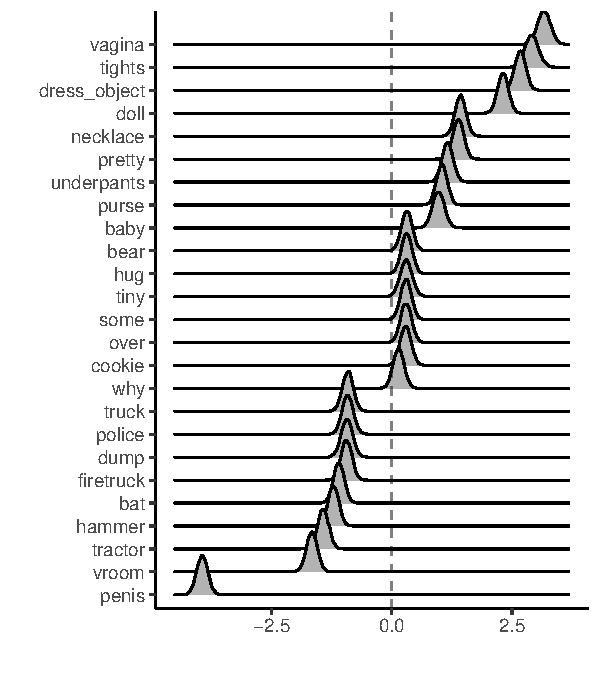
\includegraphics[width=\linewidth]{figs/smGLIMMER_sex_prodWS} 

}

\caption[GLIMMER plot of a sample of CDI:WS words from the sex bias model]{GLIMMER plot of a sample of CDI:WS words from the sex bias model. Words at the top are easier to learn for females, while those at the bottom are easier for males.}\label{fig:sex-glimmer}
\end{figure}
\end{CodeChunk}

\begin{CodeChunk}
\begin{figure}[H]

{\centering 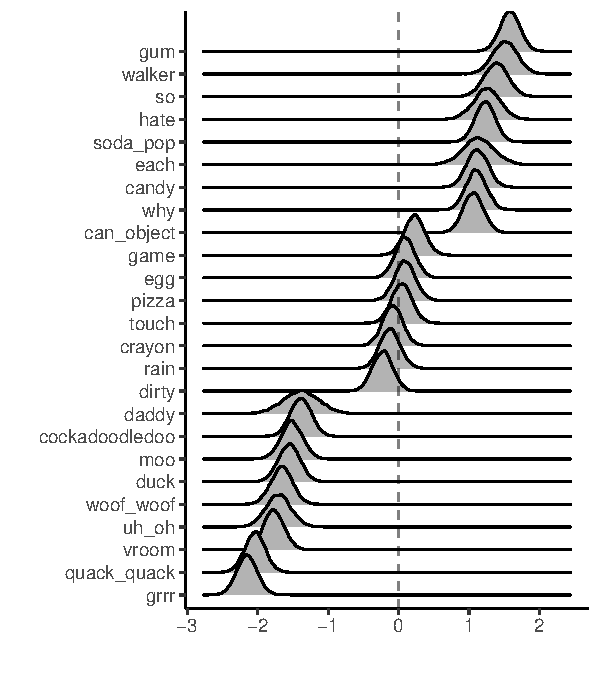
\includegraphics[width=\linewidth]{figs/smGLIMMER_ses_prodWS} 

}

\caption[GLIMMER plot of a sample of CDI:WS words from the SES bias model]{GLIMMER plot of a sample of CDI:WS words from the SES bias model. Words at the top are easier to learn for children from low-SES families, while those at the bottom are easier for those from high-SES families.}\label{fig:ses-glimmer}
\end{figure}
\end{CodeChunk}

\begin{CodeChunk}
\begin{figure}[H]

{\centering 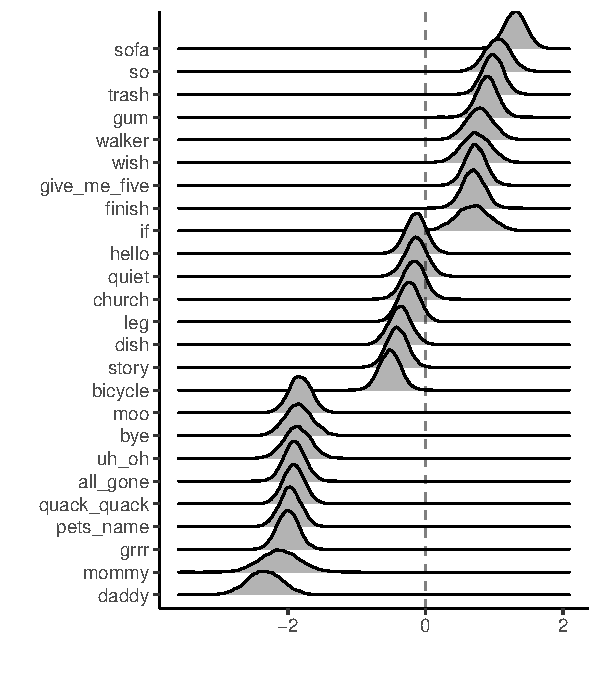
\includegraphics[width=\linewidth]{figs/smGLIMMER_eth_prodWS} 

}

\caption[GLIMMER plot of a sample of CDI:WS words from the ethnicity bias model]{GLIMMER plot of a sample of CDI:WS words from the ethnicity bias model. Words at the top are easier to learn for children from low-SES families, while those at the bottom are easier for those from high-SES families.}\label{fig:eth-glimmer}
\end{figure}
\end{CodeChunk}

\hypertarget{discussion}{%
\section{Discussion}\label{discussion}}

\hypertarget{acknowledgements}{%
\section{Acknowledgements}\label{acknowledgements}}

Place acknowledgments (including funding information) in a section at
the end of the paper.

\hypertarget{references}{%
\section{References}\label{references}}

\setlength{\parindent}{-0.1in} 
\setlength{\leftskip}{0.125in}

\noindent

\hypertarget{refs}{}
\leavevmode\hypertarget{ref-Baker2001}{}%
Baker, F. B. (2001). \emph{The basics of item response theory}. ERIC.

\leavevmode\hypertarget{ref-bornstein2016stability}{}%
Bornstein, M. H., Hahn, C.-S., \& Putnick, D. L. (2016). Stability of
core language skill across the first decade of life in children at
biological and social risk. \emph{Journal of Child Psychology and
Psychiatry}, \emph{57}(12), 1434--1443.

\leavevmode\hypertarget{ref-R-mirt}{}%
Chalmers, R. P. (2012). mirt: A multidimensional item response theory
package for the R environment. \emph{Journal of Statistical Software},
\emph{48}(6), 1--29. \url{http://doi.org/10.18637/jss.v048.i06}

\leavevmode\hypertarget{ref-fenson1994}{}%
Fenson, L., Dale, P. S., Reznick, J. S., Bates, E., Thal, D. J.,
Pethick, S. J., \ldots{} Stiles, J. (1994). Variability in early
communicative development. \emph{Monographs of the Society for Research
in Child Development}, i--185.

\leavevmode\hypertarget{ref-Fenson2007}{}%
Fenson, L., Marchman, V. A., Thal, D. J., Dale, P. S., Reznick, J. S.,
\& Bates, E. (2007). \emph{MacArthur-Bates Communicative Development
Inventories: User's guide and technical manual (2nd ed.)}. Baltimore,
MD: Brookes.

\leavevmode\hypertarget{ref-frank2017}{}%
Frank, M. C., Braginsky, M., Yurovsky, D., \& Marchman, V. A. (2017).
Wordbank: An open repository for developmental vocabulary data.
\emph{Journal of Child Language}, \emph{44}(3), 677.

\leavevmode\hypertarget{ref-frank2021}{}%
Frank, M. C., Braginsky, M., Yurovsky, D., \& Marchman, V. A. (2021).
\emph{Variability and consistency in early language learning: The
wordbank project}. MIT Press.

\leavevmode\hypertarget{ref-holland1993differential}{}%
Holland, P. W., \& Wainer, H. (1993). \emph{Differential item
functioning}. Routledge.

\leavevmode\hypertarget{ref-kachergis2021cat}{}%
Kachergis, G., Marchman, V. A., Dale, P., Mankewitz, J., \& Frank, M. C.
(2021). Online computerized adaptive tests (cat) of children's
vocabulary development in english and mexican spanish.

\leavevmode\hypertarget{ref-mayor2019}{}%
Mayor, J., \& Mani, N. (2019). A short version of the MacArthur-Bates
Communicative Development Inventories with high validity. \emph{Behavior
Research Methods}, \emph{51}(5), 2248--2255.

\leavevmode\hypertarget{ref-petersen2018gender}{}%
Petersen, J. (2018). Gender difference in verbal performance: A
meta-analysis of united states state performance assessments.
\emph{Educational Psychology Review}. Springer.

\leavevmode\hypertarget{ref-reckase2009}{}%
Reckase, M. D. (2009). Multidimensional item response theory models. In
\emph{Multidimensional item response theory} (pp. 79--112). Springer.

\leavevmode\hypertarget{ref-schwab2016}{}%
Schwab, J. F., \& Lew-Williams, C. (2016). Language learning,
socioeconomic status, and child-directed speech. \emph{WIREs Cognitive
Science}, \emph{7}, 264--275. \url{http://doi.org/10.1002/wcs.1393}

\leavevmode\hypertarget{ref-stenhaug2021treading}{}%
Stenhaug, B., Frank, M. C., \& Domingue, B. (2021). Treading carefully:
Agnostic identification as the first step of detecting differential item
functioning.

\bibliographystyle{apacite}


\end{document}
